\section{Evaluation and critical appraisal}
\label{s:evaluation}
\subsection{Sensors energy measurements}
\begin{figure}[H]
\centering
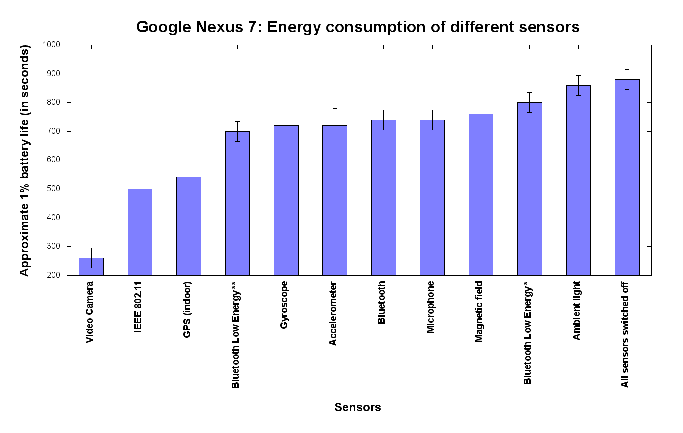
\includegraphics[scale=1.5]{plots/google_nexus_7.eps}
\caption{Google Nexus 7: Energy  consumption of different sensors.}
\end{figure}
The issue: Bluetooth vs Bluetooth LTE\\
	new functionality-> prints a lot of logs -> not energy-efficient\\

\begin{figure}[H]
\centering
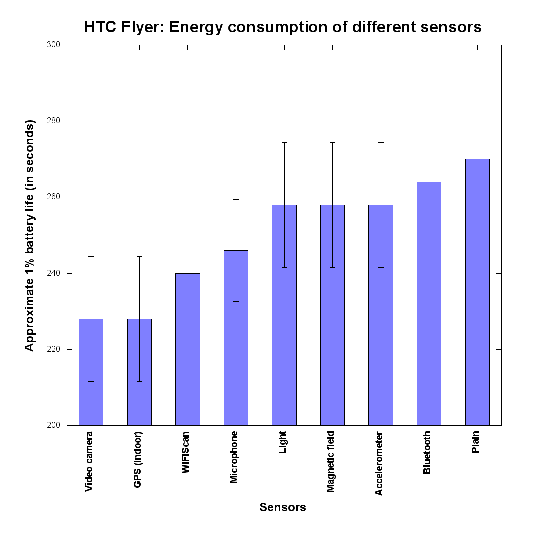
\includegraphics[scale=1.5]{plots/htc_flyer.eps}
\caption{HTC Flyer: Energy  consumption of different sensors.}
\end{figure}

\begin{figure}[H]
\centering
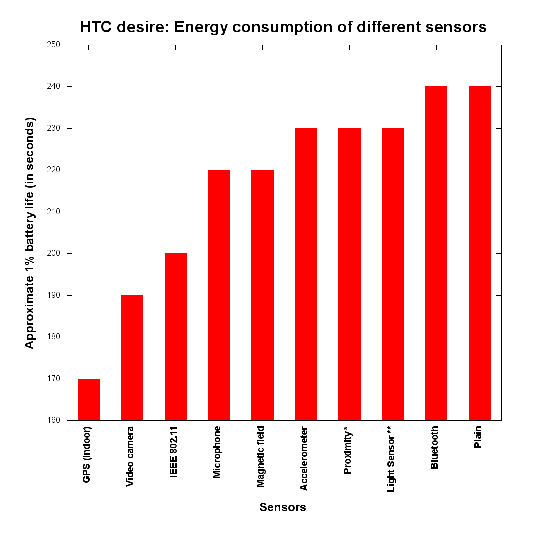
\includegraphics[scale=1.5]{plots/htc_desire.eps}
\caption{HTC Desire: Energy  consumption of different sensors.}
\end{figure}

physical sensors are always in the group of cheapest \\

Bluetooth - proximity the same, the cheapest group\\
				exactly what industry does\\
				References to beacons etc.\\

microphone good results as well, people try to utilize it(research community)\\
				SurroundSense \cite{azizyan:surroundsense}\\
				however it's not always the cheapest\\
				
				
"the order" differs among devices\\
	gives the reason for online measurement\\
	disallows the usage of power models\\
		(need to look further into how they are built)\\
		related to fragmentation problem?!\\
								
\subsection{Sensy}
\subsection{Conclusions}